\documentclass[10pt]{article}

\usepackage[margin=0.75in]{geometry}
\usepackage{amsmath,amsthm,amssymb}
\usepackage{xcolor}
\usepackage{cancel}
\usepackage{graphicx}
\usepackage{changepage}
\usepackage{circuitikz}
\usepackage{pgfplots}
\usepackage{physics}
\usepackage{hyperref}
\usepackage{siunitx}
\usepackage{fontspec}
\usepackage{relsize}
\usepackage{subfig}
\usepackage{todonotes}
\usepackage{multicol, multirow, booktabs}
\usepackage[breakable]{tcolorbox}
\usepackage[inline]{enumitem}

\theoremstyle{definition}
\newtheorem{problem}{Problem}
\newtheorem{soln}{Solution}

\pgfplotsset{compat=newest}
\usetikzlibrary{lindenmayersystems}
\usetikzlibrary{arrows}
\usetikzlibrary{calc}
\usetikzlibrary{positioning, fit}
\usetikzlibrary{3d, perspective}

\definecolor{incolor}{HTML}{303F9F}
\definecolor{outcolor}{HTML}{D84315}
\definecolor{cellborder}{HTML}{CFCFCF}
\definecolor{cellbackground}{HTML}{F7F7F7}
\newcommand{\ui}{\hat{i}}
\newcommand{\uj}{\hat{j}}
\newcommand{\uk}{\hat{k}}
\newcommand{\ux}{\hat{x}}
\newcommand{\uy}{\hat{y}}
\newcommand{\uz}{\hat{z}}
\newcommand{\primed}[1]{#1^\prime}
\pgfdeclarelayer{background}  
\pgfsetlayers{background,main}
\AtBeginDocument{\RenewCommandCopy\qty\SI}

\makeatletter
\newcommand{\boxspacing}{\kern\kvtcb@left@rule\kern\kvtcb@boxsep}
\makeatother
\newcommand{\prompt}[4]{
    \ttfamily\llap{{\color{#2}[#3]:\hspace{3pt}#4}}\vspace{-\baselineskip}
}

\newcommand{\thevenin}[2]{
  \begin{center}
    \begin{circuitikz} \draw
      (0,0) -- (2,0) to[battery1, l_=$V_{Th}\eq#1$] (2,2) 
      to[resistor, l_=$R_{Th}\eq#2$] (0,2)
      ;
      \draw [o-] (-.07,2.079);
      \draw [o-] (-.07,0.079);
    \end{circuitikz}
  \end{center}
}

\newcommand{\norton}[2]{
  \begin{center}
    \begin{circuitikz} \draw
      (0,0) -- (3,0) to[american current source, l_=$I_{N}\eq#1$] (3,2) -- (0,2) (2,0)
      to[resistor, l=$R_{N}\eq#2$] (2,2)
      ;
      \draw [o-] (-.07,2.079);
      \draw [o-] (-.07,0.079);
    \end{circuitikz}
  \end{center}
}

\DeclareMathOperator{\Div}{div}
\DeclareMathOperator{\Curl}{curl}

\newcommand{\highlight}[1]{\colorbox{yellow}{$\displaystyle #1$}}

\newcommand{\ti}[1]{\widetilde{#1}}

\newcommand{\bv}[1]{\mathbf{#1}}

\title{Physics 3130H: Assignment I}
\author{Jeremy Favro (0805980) \\ Trent University, Peterborough, ON, Canada}
\date{\today}

\begin{document}
\maketitle

% PROBLEM 1
\begin{problem}
A Skier weighing $\qty{90}{\kilo\gram}$ starts from rest down a hill inclined at $\qty{17}{\degree}$.
He skis $\qty{100}{\meter}$ down the hill and then coasts for $\qty{70}{\meter}$ along level snow until he stops.
Find the coefficient of kinetic friction between the skis and the snow. What is his velocity when he reaches the bottom of the hill?
\end{problem}
\begin{soln}
  On the hill we can use conservation of energy to find the velocity the skier will have at the bottom of the slope.
  At the top of the hill the skier has potential energy
  $$U=mgh=100mg\sin(17)$$
  and at the bottom all of this will have been converted into kinetic energy or lost to friction as work,
  $$\frac{1}{2}mv^2=mgh-100\mu_kmg\implies v=\sqrt{2g(h-100\mu_k)}$$
  where we've taken the positive root implicitly because the skier should not have negative velocity.
  Now we have sufficient initial conditions to investigate the flat part of the problem, (by shifting our origin) $v(t=0)=v(x=0)=\sqrt{2g(h-100\mu_k)}$ and $x(t=0)=0$.
  Our equation of motion in this region is
  $$F=m\ddot{x}=\mu_kN=-mg\mu_k\implies \frac{d^2x}{dt^2}=-g\mu_k$$
  which we rewrite using $\frac{d^2x}{dt^2}=\frac{dv}{dt}=\frac{dv}{dx}\frac{dx}{dt}=v\frac{dv}{dx}$ as
  $$v\frac{dv}{dx}=-g\mu_k\implies v^2/2=-g\mu_kx+C_1\implies v=\sqrt{C_1-2g\mu_kx}.$$
  applying $v(x=0)=\sqrt{2g(h-100\mu_k)}$ here,
  $$v(0)=\sqrt{C_1}=\sqrt{2g(h-100\mu_k)}\implies C_1=2g(h-100\mu_k)\implies v(x)=\sqrt{2g(h-100\mu_k-\mu_kx)}.$$
  Now we know that $v(70)=0$ so
  $$v(70)=\sqrt{2g(h-100\mu_k-70\mu_k)}=0\implies \mu_k=\frac{h}{170}$$
  so
  $$\frac{h}{170}=\frac{100\sin(17)}{170}\approx 0.17$$
  now we just substitute this into our initial condition to determine that the skiers velocity at the bottom of the hill is
  $$v(x=0)=\sqrt{2g(h-100\frac{100\sin(17)}{170})}=\sqrt{2g(100\sin(17)-\frac{10000\sin(17)}{170})}\approx \qty{15.4}{\meter\per\second}$$
\end{soln}
\newpage

% PROBLEM 2
\begin{problem}~
\begin{enumerate}[label=(\alph*)]
  \item If a projectile is fired from the origin of the coordinate system with an initial velocity $v_0$ and
        in a direction making an angle $\alpha$ with the horizontal, calculate the time required for the projectile
        to cross a line passing through the origin and making an angle $\beta < \alpha$ with the
        horizontal.
  \item When a projectile is fired with an initial
        speed of $v_0$, it passes through the points $P$ and
        $Q$ which are at a distance $h$. Find the distance
        between $P$ and $Q$ in the figure
\end{enumerate}
\begin{center}
  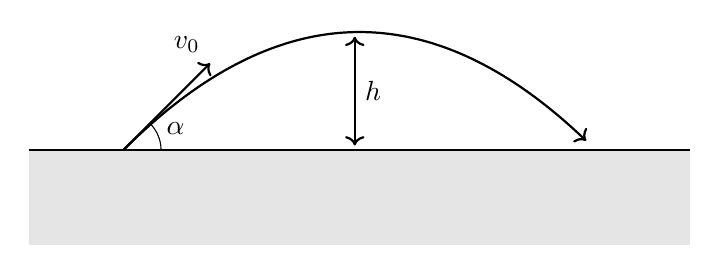
\begin{tikzpicture}[scale=1.2]
    \fill[gray!20] (-1,-1) rectangle (6,0);
    \draw[thick] (-1,0) -- (6,0);
    \draw[<->, thick] (2.45,0.05) -- (2.45,1.25-0.05) node[midway, right]{$h$};


    \draw[thick, ->, domain=0:4.9, smooth, variable=\t]
    plot[samples=100] ({\t}, {\t*(1-(1/5)*\t)});

    \draw[->, thick, rotate=45] (0,0) -- (1.3,0) node[above left] {$v_0$};

    \draw (0.4,0) arc[start angle=0, end angle=45, radius=0.4,dashed];
    \draw[draw=none, rotate=22.5] (0,0) -- (0.6,0) node {$\alpha$};
    \draw[dotted, thick] (0,0) -- (0.7,0);
  \end{tikzpicture}
\end{center}
\end{problem}
\begin{soln}~
  \begin{enumerate}[label=(\alph*)]
    \item To do this we'll need to find the point of intersection between $y_p(x)$, the trajectory of the projectile, and $y_l(x)=\tan(\beta)x$, the given line.
          To do this we solve the equations of motion for both $y(t)$ and $x(t)$. Starting with $x$,
          \begin{align*}
            F_x      & =m\ddot{x}=0 \\
            \implies & \dot{x}=C    \\
            \implies & x(t)=Ct+C_1
          \end{align*}
          and because $x(0)=0$ and $\dot{x}(0)=v_{0x}$, $C_1=0$ and $C=v_{0x}$ so $x(t)=v_{0x}t$. Now for $y(t)$,
          \begin{align*}
            F_y      & =m\ddot{y}=-mg            \\
            \implies & \dot{y}=-gt+C             \\
            \implies & y=-\frac{gt^2}{2}+Ct+C_1.
          \end{align*}
          Applying initial conditions again we get that $y(t)=-\frac{gt^2}{2}+v_{0y}t$. We then solve for $t(x)=\frac{x}{v_{0x}}$ and substitute this into $y(t)$ to obtain
          $$y(x)=-\frac{gx^2}{2v_{0x}^2}+\frac{v_{0y}x}{v_{0x}}.$$
          Now we just solve
          $$\tan(\beta)x=-\frac{g}{2v_{0x}^2}x^2+\frac{v_{0y}}{v_{0x}}x\implies \frac{2v_{0x}}{g}\left[v_{0x}\tan(\beta)-v_{0y}\right]=x$$

    \item To do this we just shift down the trajectory by $h$ so that $P$ and $Q$ are zeroes, so
          \begin{align*}
            0           & =-\frac{g}{2v_{0x}^2}x^2+\frac{v_{0y}}{v_{0x}}x-h                                                                                                                 \\
            \implies  x & =\frac{-\frac{v_{0y}}{v_{0x}}\pm\sqrt{\left(\frac{v_{0y}}{v_{0x}}\right)^2-4\left(-\frac{g}{2v_{0x}^2}\right)\left(h\right)}}{2\left(-\frac{g}{2v_{0x}^2}\right)} \\
                        & =\frac{v_{0y}v_{0x}\mp v_{0x}\sqrt{2gh+v_{0y}^2}}{g}
          \end{align*}
          then we can take the difference $Q-P$. With $Q$ being the greater,
          $$\frac{v_{0y}v_{0x}+ v_{0x}\sqrt{2gh+v_{0y}^2}}{g}-\frac{v_{0y}v_{0x}- v_{0x}\sqrt{2gh+v_{0y}^2}}{g}=\frac{2v_{0x}\sqrt{2gh+v_{0y}^2}}{g}$$

  \end{enumerate}
\end{soln}

% PROBLEM 3
\begin{problem}
A particle is under the influence of a force $F=-kx+\frac{k}{\alpha}x^3$, where $k$ and $\alpha$
are constants and $k$ is positive.
\begin{enumerate}[label=(\alph*)]
  \item Determine $U(x)$ and plot $U(x)$ as a function of x using
        computer graphing tools (if you use python, three cheers
        to you).
  \item Look at the figure carefully. Determine the
        energy $E_1$ in terms of $k$ and $\alpha$, based on the discussion
        we had in the class.
  \item If the particle has the energy $E_2$
        discuss the motion of the particle.
\end{enumerate}
\end{problem}
\begin{soln}~
  \begin{enumerate}[label=(\alph*)]
    \item $$U(x)=\int F\,dx=\int -kx+\frac{k}{\alpha}x^3\,dx=-\frac{k}{2}x^2+\frac{k}{4\alpha}x^4$$
          \begin{center}
            \begin{tikzpicture}
              \begin{axis}[
                  xmin=-2, xmax=2,
                  ymin=-0.5, ymax=1,
                  domain=-2:2,
                  samples=500
                ]
                \addplot [mark=none, blue] {-(2.5/2)*x^2+(2.5/(4*0.3))*x^4};
              \end{axis}
            \end{tikzpicture}
          \end{center}
    \item Look at the figure carefully. Determine the
          energy $E_1$ in terms of $k$ and $\alpha$, based on the discussion
          we had in the class.
    \item If the particle has the energy $E_2$
          discuss the motion of the particle.
  \end{enumerate}
\end{soln}
\end{document}